\begin{figure}[]
    \centering
    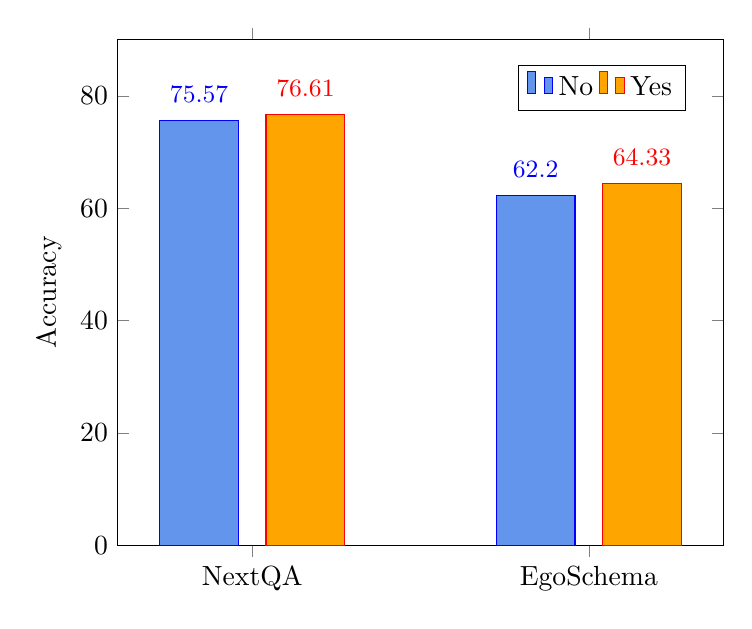
\begin{tikzpicture}
        \begin{axis}[
            ybar=0.35cm,
            bar width=1cm,
            % width=\textwidth,
            height=8cm,
            ylabel={Accuracy},
            symbolic x coords={NextQA, EgoSchema},
            xtick=data,
            % xlabel={Datasets},
            ymin=0,
            ymax=90,
            enlarge x limits=0.4,
            legend style={
                 at={(0.8, 0.95)},
                 anchor=north,
                 legend columns=-1
                 },
            nodes near coords,
            every node near coord/.append style={font=\small, yshift=3pt},
            %title={Scores by Dataset and Question Condition}
        ]
            \addplot+[ybar, fill=CornflowerBlue] 
                coordinates {(NextQA,75.57) (EgoSchema,62.20)};
            \addplot+[ybar, fill=Orange] 
                coordinates {(NextQA,76.61) (EgoSchema,64.33)};
            \legend{No, Yes}
        \end{axis}
    \end{tikzpicture}
    \caption{Question-Conditioned Token Selection.}
    % \vspace{-10mm}
    \label{fig:question condition}
\end{figure}
